%\documentclass[draft]{ws-procs11x85}
%\documentclass[square]{ws-procs11x85}
\documentclass{ws-procs11x85}

\begin{document}

\title{Paper Title}

\author{A. B. AUTHOR$^*$ and C. D. AUTHOR}

\address{University Department, University Name,\\
City, State ZIP/Zone, Country\\
$^*$E-mail: ab\_author@university.com\\
www.university\_name.edu}

\author{A. N. AUTHOR}
 
\address{Group, Laboratory, Street,\\
City, State ZIP/Zone, Country\\
E-mail: an\_author@laboratory.com}

\begin{abstract}
Here should come the abstract.
\end{abstract}

\keywords{keyword 1; keyword 2; keyword 3;}

\bodymatter

\section{Introduction} 
\label{introduction}

Studying interactions between proteins has been of utmost importance in
understanding how proteins work collectively to govern cellular
function\cite{schwikowski,uetz}. Such collection of interactions among
proteins is called a protein interaction network. Mathematically, a protein
interaction network is often modeled as an edge-weighted undirected graph where
each node denotes a protein and each edge represents an interaction between a
pair of proteins. The weight of an edge denotes the level of confidence that
this interaction truly exists.

One of the key outcomes of computational analysis of protein interaction
networks is identification of signaling pathways. A signaling pathway is a
series of proteins in which each protein participates in transmitting
biological information by modifying its successor through an
interaction. Thus, signaling pathways can be viewed as simple paths in protein
interaction networks\cite{kelley}.

The confidence value of an interaction between two proteins is often considered
as the probability that a signal is transmitted between those two proteins.
Thus, the probability that a signal moves through a pathway is the product of
the confidence values of its constituting interactions. Under this model, Scott
et al. conjectured that a signal tends to move through the most probable
pathway\cite{scott}. They showed that such pathways yield signaling pathways,
and thus help in reconstructing signaling networks. Following defines the
problem of identifying the most probable pathway in a protein interaction
network.

\paragraph{Problem} Consider a protein interaction network $(V, E, \lambda)$ where
$V$ denotes the set of proteins, $E = \{(u, v) | u,v \in V\}$ denotes the set of
interactions, and the function $\lambda(): E \Rightarrow [0, 1]$  denotes interaction
confidence for each interaction in E. Assume that we are given a set of starting
proteins $S \subseteq V$ and a set of target proteins $T \subseteq V$. Given a
path length denoted by a positive integer $m$, the problem is to find a simple
path $\Phi = v_1 \rightarrow v_2 \rightarrow \ldots \rightarrow v_m$, where
$\prod_{i=1}^{m-1} \lambda(v_i, v_{i+1})$ is maximum among all paths with $v_1 \in
S$, $v_m \in T$ and $v_i \in V \forall i \in \{1, 2, \ldots , m\}$.

The problem above is equivalent to finding a simple path $\phi = v_1 \rightarrow
v_2 \rightarrow \ldots \rightarrow v_m$, where $\sum_{i=1}^{m-1} -$log
$\lambda(v_i, v_{i+1})$ is minimum among all paths with $v_1 \in
S$, $v_m \in T$ and $v_i \in V \forall i \in \{1, 2, \ldots , m\}$. The
traveling-salesman problem is polynomial-time reducible to this
problem\cite{scott}; therefore it is NP-hard. They developed a method using a
technique devised by Alon et al.\cite{alon}, called \textit{color-coding}. The
basic idea of this method is to randomly assign each node in the graph one of
$m$ different colors, and search for an optimal pathway in the restricted
domain of colorful pathways. A pathway is colorful if and only if all of its
nodes are in different color. Finding a colorful path is computationally much
cheaper than finding a path without assigning colors. The drawback is that the
optimal path may not be colorful in a random color assignment. If that happens,
the color coding method fails to find the true optimal result. To deal with
this, color coding method repeats the coloring process for several iterations.
The confidence in the optimality of the result monotonically increases with each
iteration until it reaches a given level of confidence that the unknown optimal
pathway was among the colorful ones in at least one of these iterations. As we
elaborate later in section \ref{background}, the confidence value depends
solely on the pathway length $m$ and does not capitalize on readily available
information such as the network topology and color assignment. As a result, the
method provides a theoretically correct but very conservative confidence value.
Hence it requires many iterations in order to achieve a given confidence level,
leading to an unnecessarily innefficient running time performance.

G{\"u}lsoy et al.\cite{gulsoy} presented an enhanced color-coding technique
called \textit{k-hop coloring}. A colored network is k-hop colorable if the
shortest path between all pairs of same-color nodes is more than $k$ hops in
length. This method exploits the network topology and the node colors to assign
the network a maximal value $k$ such that the network is $k$-hop colorable.
This additional piece of information allows for higher success probability at
each iteration, yielding fewer iterations than that by Scott et al. However,
subnetworks with high connectivity quickly diminish the ability to $k$-hop
color the whole network for large values of $k$. For example, a network
containing a clique of size $m$ cannot be colored with ($m-1$)-hop coloring
using $m$ colors\cite{gulsoy}.

\paragraph{Contribution} In this paper, we consider the problem of finding
signaling pathways in protein interaction networks. We develop a new coloring
method that overcomes the bottlenecks of exisiting coloring methods by Scott et
al.\cite{scott} and G{\"u}lsoy et al\cite{gulsoy}. Our contribution comes from a
deeper understanding of the relation between network topology, random color
assignment and confidence value. We assign a $k$ value to each node
individually by studying the colors of all the nodes in the network. The $k$
value of a node $v$ at an iteration indicates that there is no other node $u$
that is reachable from $v$ in $k$ hops such that both $u$ and $v$ have the same
color. For each node, the $k$ value is the largest integer that satisfies the
above constraint. Thus, different nodes in the network may have different $k$
values. We also study how this reflects on the resulting success probability for
each iteration. Given different $k$ values for each node on a pathway, we show
how to obtain a bound on success probability.

Based on these findings, We present a new method for detecting signaling
pathways in protein interaction networks using an enhanced k-hop coloring
technique. Given the parameter pathway length $m$, we start by randomly
assigning one of $m$ colors to each node in the graph, we then extract the
optimal colorful pathway. We then calculate our new bound on success
probability. We repeat this process until the cumulative success probability is
at least equal to a given confidence level. Although our theoretical findings
are based on assuming the knowledge of the $k$ values assigned to the unknown
global optimal pathway, we empirically demonstrate that the local optimal
pathway extracted from the domain of colorful pathways yields correct
confidence values.

The coloring methods developed by G{\"u}lsoy et al.\cite{gulsoy} and Scott et
al.\cite{scott} yield special cases of our method. The first method is our
method in the special case of all the nodes in the network having the same $k$
value. The second method is our method in the special case of all the nodes in
the network having $k$ value $= 0$. Hence, our method is guaranteed to perform
at least as good as both of them in these special cases, and better in the
general case.

We provide validation experiments to test the biological significance of our
results. We use \textit{weight p-value} and \textit{functional enrichment} as
validation measures. We also compare the performance of our method against the
one presented by Scott et al.\cite{scott} with respect to how fast our method
reaches a given confidence level as opposed to theirs.

The rest of the paper is organized as follows. Section 2 discusses the
background and related work. Section 3 explains how to obtain a tighter bound on
success probability and describes our enhanced k-hop coloring method. Section 4
shows the experiments performed and their results. Section 5 is the conclusion
of the paper.


\section{Background}
\label{background}

A number of methods have been developed so far to identify signaling networks
from protein interaction networks. These methods differ in the way they
formulate the problem. Among them, Zhao et al.\cite{zhao} formulated a linear
optimization problem that finds the maximum weighted subnetwork with a given
size. The main difference of this approach from this paper is that it is
concerned with finding signaling subnetworks rather than linear pathways.
Kelley et al.\cite{kelley} detected conserved signaling pathways between
related organisms by performing global alignment between their protein
interaction networks. They scored each pathway in terms of the probability of
true homology between aligned pair of proteins, as well as the probability of
true interactions between pairs of proteins along the pathway. Shlomi et
al.\cite{shlomi} introduced QPath, a method for querying protein interaction
networks for pathways using known homologous pathways as queries. They scored
results based on their similarity to the query, number of insertions and
deletions used, as well as the reliability of their interactions. Both Kelley
et al.\cite{kelley} and Shlomi et al.\cite{shlomi} are comparative methods.
They require knowledge of multiple interaction networks. Thus, they solve a
related, yet different, computational problem than the one considered in this
paper.

Lu et al.\cite{lu} presented a divide-and-conquer algorithm to find signaling
subnetworks in protein interaction networks. They recursively partitioned the
network into two sets of vertices, enumerated substructures present in each
set, and then built larger subnetworks from them. They assumed that all edges
have the same weight. They scored the resulting subnetworks based on the
similarity of expression profiles of their nodes to the given source and
destination nodes. This method formulates a different objective. It aims to
detect paths whose proteins are highest in expression similarity, and thus it
does not utilize the confidence in the interactions.

Steffen et al.\cite{steffen} studied detecting signaling pathways in protein
interaction networks as guided by expression data. They listed all pathway
candidates in a protein interaction network using exhaustive search. They
scored each candidate based on how similar the expression profiles of its
genes are. Bebek et al.\cite{bebek} presented a method called PathFinder for
finding new signaling pathways using association rules of known ones. They
started with mining association rules for known pathways, guided by the
knowledge of functional annotations of their proteins. They then performed an
exhaustive search for candidate pathways. From these candidates, they selected
the ones having at least a certain number of the known association rules and an
average interaction weight above a given threshold. The drawback of both of
these methods is that the time complexity of exhaustive graph search is
exponential in terms of the network size, and hence is very inefficient.

Gitter et al.\cite{gitter} presented a method for discovering signaling
pathways by adding edge orientation to protein interaction networks. They
selected an optimal orientation of all edges in the network that maximizes the
weights of all satisfied length-bound paths. They say a path is satisfied if it
follows the same direction along its edges from a source node to a destination node.
They proved that this problem is NP-hard. They provided two approximation
algorithms for it based on available solution methods for weighted Boolean
satisfiability, and a third algorithm based on probabilistic selection. As
shown in their results, these methods do not scale well with increasing the
number of source and destination nodes and the required path length.

The closest studies to that presented in this paper are those by Scott et
al.\cite{scott} and G{\"u}lsoy et al\cite{gulsoy}. The former detected signaling
pathways in protein interaction networks using color coding. The latter
developed topology-aware color coding for network alignment. We describe both
methods in detail in section \ref{introduction}. Both methods run multiple 
coloring iterations. Let us denote the probability that the coloring at an
iteration is successful (i.e. true optimal path is colorful) with $P_s$. The
probability that at least one out of $r$ iterations is successful is $1 - (1 -
P_s)^r$. Following from this, in order to insure confidence of at least
$\epsilon$ ($0 \leq \epsilon \leq 1$), they run $r$ iterations, such that $1 -
(1 - P_s)^r \geq \epsilon$. Both methods calculate success probability as
\begin{equation}
P_s = \frac{m!}{N_c}
\label{ps}
\end{equation}
where $N_c$ is the number of coloring assignments possible for the optimal
pathway. They differ in the way they compute $N_c$. Scott et al.\cite{scott}
calculated $N_c = m^m$. G{\"u}lsoy et al.\cite{gulsoy} calculated a bound $N_c
\leq (m - k)^{m - k} \prod_{i=0}^{k-1} (m - i)$ where $k$ is the value assigned
to the network such that it is $k$-hop colorable. Notice that in equation
\ref{ps}, smaller values for $N_c$ are desirable. This is because small values
for $N_c$ increase success probability, and thus reduces the number of
iterations needed to attain a given confidence level $\epsilon$. This paper
develops a novel method that computes a much smaller upper bound on $N_c$ than
both Scott et al. and G{\"u}lsoy et al., hence a better lower bound on $P_s$.

\section{Methods}
In this section, we start by properly formulating the problem and defining
common terms that we use in our methods. We then present new thoughts about
pathway detection using color coding. We study the opportunity of more involving
of network topology in our calculation to obtain a better success probability,
and hence needing less number of iterations and improving performance. Last, we
present an enhanced color-coding method for detecting pathways in protein
interaction networks.

\subsection{Success Probability: a Tighter Bound}
Our key contribution is to establish the relationship among network topology,
node colors and sucess probability in a single iteration of color coding. In
this section, we focus on one coloring iteration and describe how we compute the
probability of success in that iteration.

Assume that we are given a protein interaction network similar to the one
described in section \ref{introduction}, denoted by $G = (V, E, w)$, where
$w(u, v) = -$log $\lambda(u, v)$. Also assume that the colors of the nodes are
already assigned in the current iteration. We denote the set of possible colors
with $\{c_1, c_2, \ldots , c_m\}$ and denote the color of node $v \in V$ with
$c(v)$.

Consider any colorful path with $m$ nodes. The number of ways to assign colors
to the nodes of that path while keeping it colorful is $m!$. Notice that this is
equal to the numerator in equation \ref{ps} for probability of success. The
denominator in that equation, denoted by $N_c$, is the total number of ways to
color that path regardless of whether it yields colorful or not. Before we
discuss how we compute $N_c$, we describe the following concepts.

\begin{arabiclist}[3]
\item $k$ neighborhood of a node. Let $v \in V$ be a node in $G$, and $k$ be a
natural number. $\Psi_k(v)$ is the set of nodes where $\forall u \in V
\backslash \{v\}$, $u \in \Psi_k(v)$ if and only if $u$ is reachable from $v$
in $k$ hops of less. We call $\Psi_k(v)$ the $k$ neighborhood of $v$. Figure
\ref{colors} shows an example of a colored network. In this example, $\Psi_1(a)
= \{d\}$ because the node $d$ is the only node that is reachable from the
node $a$ in 1 hop (or less). Similarly, $\Psi_1(f) = \{c, e\}$, $\Psi_2(a) =
\{d, e\}$ and $\Psi_2(f) = \{c, e, b, d\}$.
\item $k_{max}$ value of a node. Let $v \in V$ be a node in $G$. $k_{max}(v)$ is
the maximal value of $k$ such that $\forall u \in \Psi_k(v)$: $c(u) \neq c(v)$.
Figure \ref{colors} also shows the $k_{max}$ values for the nodes in the
network. For example, $\forall u \in \Psi_1(f) = \{c, e\}$, $c(u) \neq
c(f)$. If we try to expand to $\Psi_2(f) = \{c, e, b, d\}$, we find that $c(d)
= c(f) = c_2$. Therefore $k_{max}(f) = 1$. Similarly, $k_{max}(a) = 3$ and
$k_{max}(b) = 0$.
\item $k_{max}$
configuration of a path. Let $\Phi = v_1 \rightarrow v_2 \rightarrow \ldots \rightarrow v_m$ be a path of length $m$ in $G$. The
$k_{max}$ configuration of $\Phi$ is the sequence $[k_{max}(v_1),
k_{max}(v_2), \ldots , k_{max}(v_m)]$.
\end{arabiclist}


\begin{figure}[h]
\centerline{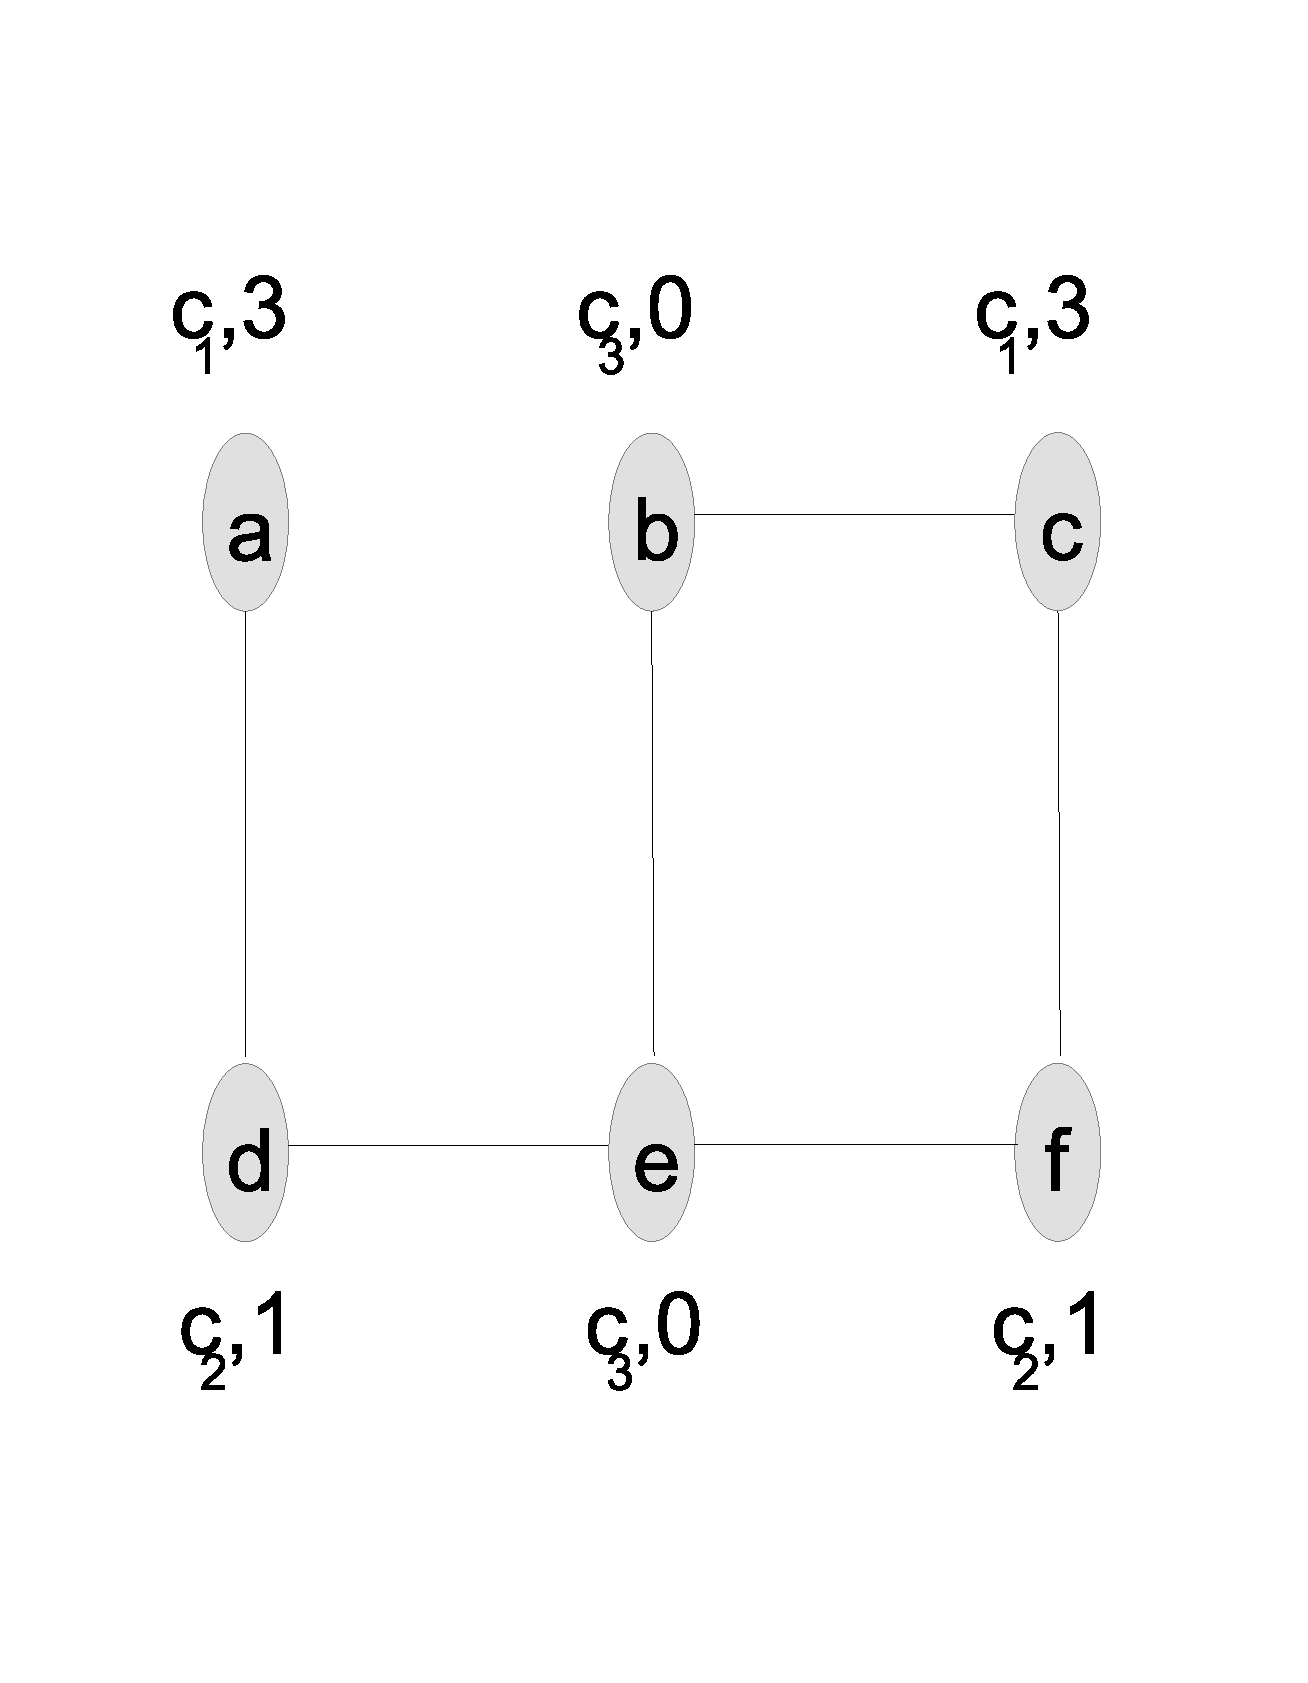
\psfig{file=colors.eps,width=9cm,height=6cm}}
\caption{(a) An example colored network. Each node carries two labels. The
label on the left is the color assigned to this node. The label on the right is
the node's $k_{max}$ value}
\label{colors}
\end{figure}



Our approach relies on individual $max\_k$ values of all nodes in an optimal
path. Assuming knowledge of the $max\_k$ configuration of the optimal path, we
use it to calculate $N_c$ under the restrictions induced by these values. We
also assume that each node in the path is not connected to any other nodes
except the ones before and after it in the path. This assumption is valid
because any more connections will only induce more coloring restrictions,
causing $N_c$ to decrease; therefore we get a solid upper bound on $N_c$, hence
a solid lower bound on $P_s$ according to equation (\ref{ps}). For a given node
$v$ in a given path, all $max\_k(v)$ nodes in either direction from $v$ are not allowed to have the same
color as $v$. We represent this rule as an unweighted constraint graph $W = (H,
L)$ where $H$ is its set of nodes and $L$ is its set of edges. $H$ contains a
node corresponding to each node in the path, and $L$ contains an edge for each
pair of nodes that are not allowed to have the same color, according to the
aforementioned rule. Figure \ref{maxk} shows an example of a path, its $max\_k$
configuration and the corresponding constraint graph $W$. The problem now
translates to calculating the value of the chromatic polynomial $P(W, m)$: the
number of ways of coloring $W$ using $m$ colors without any pair of adjacent
nodes having the same color. We calculate this value using the following
edge-contraction recursive rule based on the fundamental reduction
theorem\cite{dong}:
\begin{equation}
P(W, m) = P(W - uv, m) - P(W / uv, m)
\label{eqchromatic}
\end{equation}
where $u$ and $v$ are any pair of adjacent nodes, $W - uv$ is the graph $W$
after removing the edge $uv$, and $W / uv$ is the graph $W$ after merging the
nodes $u$ and $v$.

\begin{figure}[h]
\centerline{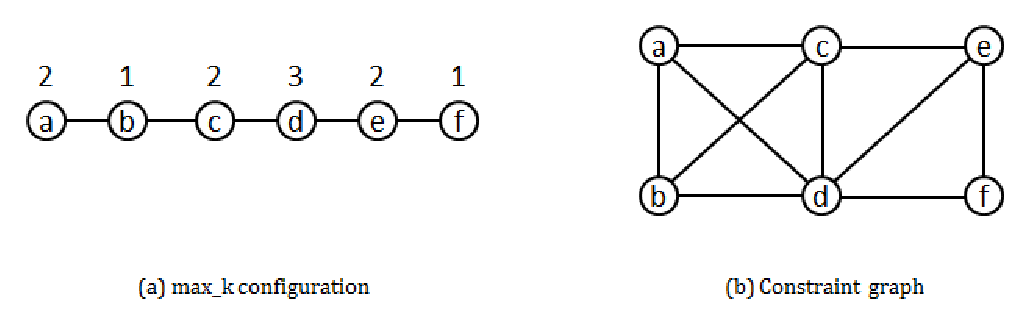
\psfig{file=maxk.eps,width=16.5cm}}
\caption{(a) An example 6-node path with its $max\_k$ configuration shown above
it. Each $max\_k$ value translates to the number of nodes that have to be of
different color on either direction. (b) The corresponding constraint graph $W$:
each pair of adjacent nodes have to be of different color. Finding the value of
the chromatic polynomial $P(W, m)$ yields the number of coloring possibilities
for the path under the given constraints.}
\label{maxk}
\end{figure}

According to this method, the value of $N_c$ for the example path shown in
Figure \ref{maxk}(a) is 5,760, while Scott et al.\cite{scott} and G{\"u}lsoy et
al.\cite{gulsoy} would respectively yield $N_c$ = 46,656 and 18,750 for the same
example. Such a decrease in the value of $N_c$ leads to an increase in the value
of $P_s$ according to equation (\ref{ps}).

\subsection{Method: Enhanced k-hop Coloring}
The approach introduced in the previous section for calculating success
probability assumes the knowledge of the $max\_k$ configuration of the optimal
path. Needless to say, this is not the case. We present a conjecture that we
can instead use the $max\_k$ configuration of the local colorful optimal path.
We empirically show that this substitution serves the purpose. Our method reports
the optimal colorful path in each iteration and computes $P_s$ based on its
$max\_k$ configuration. We also keep a heap of the top 100 reported paths to
cover the possibility of a pathway having a suboptimal score. The method is
detailed as follows:
\begin{arabiclist}[9]
\item Initializations:
	\begin{romanlist}[iii]
	\item $M \Leftarrow \{1, 2, . . . , m\}$: the set of all m colors.
	\item $P \Leftarrow 0$: overall success probability.
	\item $H \Leftarrow \{\}$: heap of top 100 paths.
	\end{romanlist}
\item $\forall v \in V$, $c(v) \Leftarrow$ a color uniformly drawn from $M$.
\item $\forall v \in V$, the minimum weight of a colorful path colored only
using $M' \subseteq M$, starting within $S$ and ending at $v$, can be
dynamically tabulated using the following recurrence\cite{scott}:
\begin{equation}
W(v, M') = \min_{u:c(u) \in (M' \backslash \{c(v)\})} W(u, M' \backslash
\{c(v)\}) + w(u, v), |M'| > 1
\end{equation}
where $W(v, \{c(v)\}) = 0$ if $v \in S$ and $\infty$ otherwise.
\item Report path $X$ whose weight $= \min_{v \in V} W(v, M)$.
\item Add $X$ to $H$.
\item Compute $N_c$ using the $max\_k$ configuration of $X$ according to the
chromatic polynomial recurrence detailed in equation (\ref{eqchromatic}).
\item Compute $P_s \Leftarrow m! / N_c$.
\item Update $P \Leftarrow 1 - (1 - P)(1 - P_s)$.
\item Repeat from step (2) until $P \geq \epsilon$.
\end{arabiclist}


\section{Experiments}

\subsection{Datasets}
Here we list the datasets used in experiments. I think we can use the MINT
datasets for multiple organisms.

\subsection{Validation Experiments}
Here we list the validation experiments we did and their results. I think we
should do some validation experiments similar to those done in Sharan's paper,
using weight p-value and functional enrichment as validitiy measures.

\subsubsection{Validation using Weight p-value}
For each dataset we use, we should obtain the 99 percent confidence optimal
pathway and compare it with optimal pathways obtained we obtain from random
networks. We generate random networks by shuffling edges of the original
network. The weight p-value is the percentage of cases where the algorithm
produces a more optimal pathway when run on one of these random networks.

\subsubsection{Validation using Functional Enrichment}
 For each dataset, we we obtain the 99 percent confidence optimal pathway and
 test its functional enrichment. For each GO term appearing on the dataset
 proteins, we count the total number of proteins annotated by it and the
 number of proteins in the resulting pathway annotated by it. We use these
 numbers, along with the total number of proteins and the number of proteins in
 the pathway, as parameters for a hypergeometric test (I still have to develop
 further understanding about the details of this test). The maximum enrichment
 value for any of the tested GO terms gives us the final functional enrichment
 p-value.

\subsection{Comparison with Sharan}
This is just a temporary title for this subsection, I'm not very sure what to
name it.

\paragraph{}
We measure the time and number of iterations needed by our method to obtain
70\%, 90\% and 99\% confidence pathways of lengths 6, 7, 8 and 9 nodes. We
compare these numbers against the ones by Sharan's method for the same cases.

\paragraph{}
We run our method for 500 iterations and measure the incremental success
probabilty against iteration number. We do this experiment many times take the
average curve. We do the same experiment using Sharan's method and obtain a
second curve. We also measure the average practical success probability, which
is the observed probability that the DP algorithm finds the optimal solution in
a certain iteration or before it. We compare the three curves targetting two
conclusions: (1) our method is experimentally solid because our calculated
success probabiilities are lower than the observed ones; and (2) our method
outperforms Sharan's method.

\section{Conclusion}
Here goes the conclusion.


\bibliographystyle{ws-procs11x85}
\bibliography{references}

\end{document}
